\documentclass[tikz,border=4pt]{standalone}
\begin{document}
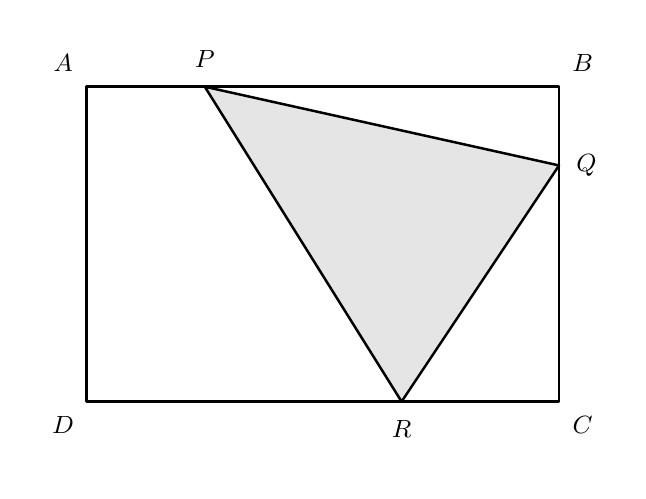
\begin{tikzpicture}[x=0.025cm,y=-0.025cm]
\path[use as bounding box] (0,0) rectangle (300,225);
\path[draw=black,fill=none,line width=0.8999999999999999pt,line join=round] (30,30) -- (270,30) -- (270,190) -- (30,190) -- cycle;
\path[draw=black,fill=gray!20,line width=0.8999999999999999pt,line join=round] (90,30) -- (270,70) -- (190,190) -- cycle;
\node[font=\small,inner sep=0pt] at (18,18) {$A$};
\node[font=\small,inner sep=0pt] at (282,18) {$B$};
\node[font=\small,inner sep=0pt] at (282,202) {$C$};
\node[font=\small,inner sep=0pt] at (18,202) {$D$};
\node[font=\small,inner sep=0pt] at (90,16) {$P$};
\node[font=\small,inner sep=0pt] at (284,70) {$Q$};
\node[font=\small,inner sep=0pt] at (190,204) {$R$};
\end{tikzpicture}
\end{document}
